\section{Design Overview}
In this section we briefly describe all the static things in our system, such like architecture, each component’s data structure, data locations, relationship of data references, etc.

We discuss the characteristics and 
main requirements for VM snapshot backup in a cloud environment.
which are different from a traditional data backup. 

\begin{enumerate}
\item {\em Cost consciousness.}
There are tens of thousands of VMs running on a large-scale cluster. 
The amount of data is so huge such that backup cost must be controlled carefully.
On the other hand, the computing resources allocated for snapshot service is very limited
because VM performance has higher priority.  
At Aliyun, it is required that while CPU and disk usage should be small or modest during backup time,
the memory footprint of snapshot service should not exceed 500MB at each node.

\item {\em Fast backup speed.}
Often a cloud has a few hours of light workload each day (e.g. midnight),  which creates an small window for automatic backup.
%But a  longer use of bandwidth and computing resource  for backup can create  noticeable  contention with the existing cloud,
%which is not preferred for cloud production system operation. 
Thus it is desirable that backup for all nodes
can be conducted in parallel and any centralized or cross-machine communication for
deduplication should not become a bottleneck.
%As a large-scale cluster hosting tens of thousand of active VMs everyday,  the amount of data
%to be processed is huge. 
%For example, in an Aliyun cluster with over 1,000 nodes and each hosts over 25 VMs, The aggreated amount of data 
 % the system must finish saving daily snapshots of all VMs in 2 hours. In our typical 1000 nodes cluster, each node hosts 25 VMs, each VM has 40GB of data on average, that translates to backup throughput of 139GB/second, or 500TB/hour.

% the system must finish saving daily snapshots of all VMs in 2 hours. In our typical 1000 nodes cluster, each node hosts 25 VMs, each VM has 40GB of data on average, that translates to backup throughput of 139GB/second, or 500TB/hour.
\item {\em Fault tolerance.}
The addition of data deduplication should not decrease the degree of
fault tolerance. It's not desirable that small scale of data failure affects the backup of many VMs.
%when users access snapshots in a recovery process. 
\end{enumerate}

There are multiple choices in designing a backup architecture  for VM snapshots.
We discuss the following design options with a consideration on their strengths and weakness.
\begin{enumerate}
\item  {\em An external and dedicated backup storage system.} 
In this architecture setting, a separate backup storage system using
the standard backup and deduplication techniques can be deployed~\cite{bottleneck08,extreme_binning09,sparseindex09}. 
This system is attached to the cloud network and every machine can periodically transfer snapshot data to 
the attached backup system. 
A key weakness of this approach is communication bottleneck between a large number of machines
in a cloud to this centralized  service.
Another weakness is that the cost of allocating separate resource for dedicated backup  can be expensive.
Since most of backup data is not used eventually, CPU and memory resource in such a backup cluster may not be fully utilized.
\item {\em A decentralized and co-hosted backup system with full deduplication.}
In this option, the backup system runs on an existing set of cluster machines.
% and a distributed storage architecture for backup allows a possible exploitation of  data locality between
%the source of data and storage location of backup data. 
The disadvantage is that 
%the backup service would compete CPU, memory, and disk resources with the other cloud services.
even such a  backup service may only use  a fraction of the existing disk storage, 
fingerprint-based search does require a significant amount of memory for fingerprint lookup of searching duplicates.
This competes memory resource  with the existing VMs.
%Decentralized deduplication is studied in ~\cite{Clements2009} and the focus is on
%block-level copy-on-write and compare-by-value techniques.

Even approximation~\cite{extreme_binning09,sparseindex09} can be used to reduce memory requirement,
one key weakness the hasn't been addressed by previous solutions is that global content sharing affects
fault isolation.
Because a content chunk is compared with a content signature collected from other users,
this artificially creates data dependency among different VM users.
% since storage for shared identical content chunks can become a failure point.
In large scale cloud, node failures happen at daily basis,
the loss of a shared block can affect many users whose snapshots share this 
data block. 
Without any control of such data sharing, we can only increase  
replication for global dataset to enhance the availability,
but this incurs significantly more cost.

%we want to isolate 
%each VM's snapshot backup as much as possible while still enjoy the benefit of deduplication.
%In large scale cloud, node faiures happen at daily basis, we don't want a problem at small scale
%to affect large amount of VMs due to data sharing.
%a key weakness of global content fingerprint comparison is that it affects fault isolation.

%2) data sharing among users for accessing common signagutes causes the system less resilient to storage failures.
%any loss of one piece of  shared data content hash and actualcontent will damange many VM snapshots, which can cause massive impacts
%on reliability of many users.

%Another point is that the previous work in signature-based comparison does not address
%load balancing for a distributed environment during parallel access.  
%Some content signatures can be extremely hot, but the machines  that  handle such signatures can become
% a bottleneck. Uncoordinated signature assignment could lead to imbalanced access workload.
\end{enumerate}


%There are multiple choices of snapshot backup design for VM images and our considerations are described
%as follows. 
%Our design considerations
%\begin{enumerate}
%\item {\bf Centralized vs. decenalized} 
%
%It is desirable to have  a decentralized architecture.
%Given a large amount of snapshot data communicated from each machine to the backup storage,
%with a distributed storage architecture for backup, one could exploit  exploit data locality between
%the source of data and storage location of data to reduce cross-platform bandwidth requirement for backup.

%execute in parallel and easy to coordinate. In fact, we want to avoid cross-node dependency at scheduling VM snapshot operations, such that no global coordinator is necessary.
%\item {Load balancing in resource consumption}: the cost of snapshot service shall be evenly distributed onto every node. We don't have a super powerful
%or stable node that can accept extra responsibility.
%\item {minimization of inter-user data dependency for fault tolerance}: we want to minimize the data dependency to a controllable level. Data deduplication means sharing of data, thus one failure at a single point may affect the snapshot service of hundreds of VMs, which is absolutely unacceptable.
%\item {Resource usage modeling and control}.
%\end{enumerate}

With these considerations in mind, we propose a decentralized backup architecture with multi-level and selective 
deduplication. This service is hosted   in the existing set of machines and resource usage is controlled
with a minimal impact to the existing applications.
The deduplication process is first conducted among snapshots within each VM
and then is conducted across VMs.  
Given the concern that searching duplicates across VMs is a global feature which can affect parallel performance
and complicate failure management,
we only eliminate the duplication of a small but popular data set while still maintaining a cost-effective deduplication ratio.
For this purpose, we exploit the data characteristics of snapshots and collect most popular data.
Data sharing across VMs is limited within this small data set such that adding replicas for it could enhance fault tolerance.
%
%in the  our studies show that there are a large amount of data unmodified in VM snapshots
%and shared among many users (e.g. OS data). The sharing pattern follows a zip-like distribution.
%With this characteristic, we can store a small amount of popular data items which coverage a large amount of
%snapshot data blocks. 
%We discuss our design and data analysis in the next section.


%This method is based on the observation of two facts in Aliyun's VM cloud: first, VM's OS disks contain 
%huge amount of operating system and software related data which is almost never modified during VM's life span. 
%Second, the duplication pattern of user generated data follows Zipf-like law, thus a tiny set of hottest data
%take up the majority of data duplication. As a result, if we extract these hot data as a common data set,
%then most of data duplication will emerge by searching in this very small scope.


%For example, In cloud storage, we are solving data deduplication problem in a different context of 
%data stream deduplication (the D2D case): our snapshot storage service is co-located with runtime VMs,
%thus we have very limited amount of system resource leave for data deduplication. For example,
%in Aliyun's 8-core, 48GB memory, 12TB VM server, there lives over 20 VMs who are hungrily competing for
%system resources: some may running map-reduce jobs, some may serving busy web requests, 
%some may storing backend databases, any behavior that affects user VMs performance or stability is unacceptable.

%To reduce the cost of deduplication, we must confine the scope of searching duplicates as much as possible,
%thus some hints are needed to tell us where the most likely duplicates would hide. 
%Several form of hints have been used in the past: many D2D systems exploits locality,
%which bases on the fact that duplicates are likely to appear in the same sequence as they have arrived before.
%Similarity is another popular hint, it suggests that two sets of data blocks may contain lots of
%duplicates if they are indetified as similar by certain similarity detection measurements.

Overall, our contributions are:
\begin{enumerate}
\item {\em CDS. parallelism, localized}
We designed a highly efficient global deduplication scheme using common data between VMs as the primary
deduplication target, which adopts to our resource-constrained production environment very well. We developed a fast
approxmation algorithm to extract the commonly used data from VM snapshot backups.

\item {\em Append Store.}
We address the problem of managing billions of small variable-sized data objects by building an append store
on top of our distributed file system (DFS). We carefully designed an efficient index data structure to 
optimize large sequential read/write requests, while minimize the cost of key to object location conversion.

\item {\em Fast Data Deletion.}
Traditional deletion in deduplication systems involves reference counting, either online or offline. Both ways
are costly due to the sharing of large amount of data objects.
We avoid this cost of data deletion with an approxmation deletion method using bloom filters.

\item {\em Fault-tolerant.}
Golbal deduplication brings data sharing across different users VM snapshots, therefore a single failure
on some data can break many VMs' snapshots. We avoid such all-to-all data dependency by restricting
the cross VM data sharing with the CDS. By taking extra care of protecting CDS data, 
the overall degree of fault tolerancy is guaranteed.

\end{enumerate}

\subsection{Design Considerations}
While this idea sounds conceptually simple, realizing it requires us to address three
significant challenges:
\begin{enumerate}
\item {\em In-cloud backup}
We decided to build 
\item {\em Inline deduplication}
Inline deduplication requires more resources and can suffer from latency issues as data is checked against metadata before being committed to disk or flagged as a duplicate.
\item {\em Data dependency}

\item {\em Backup speed}

\end{enumerate}
\subsection{Architecture Overview}
Our architecture is built on the Aliyun platform which provides the largest public VM cloud in China 
based on Xen~\cite{Xen2003}. A typical VM cluster in our cloud environment
consists of from hundreds to thousands of physical machines, each of which can
host tens of VMs.

A GFS-like distributed file system holds the responsibility of managing physical disk storage
in the cloud. All data needed for VM services, which include runtime VM disk images and snapshot backup data,
reside in this distributed file system.
During the VM creation, a user chooses her flavor of OS distribution and the cloud system 
copies the corresponding pre-configured base VM image to her VM as the OS disk, 
and an empty data disk is created and mounted onto her VM as well. 
All these virtual disks are represented as virtual machine image files in our
underline runtime VM storage system. The runtime I/O between virtual machine and its virtual
disks is tunneled by the virtual device driver (called TapDisk\cite{Warfield2005} at Xen). To avoid network latency and congestion, 
our distributed file system place the primary replica of VM's 
image files at physical machine of VM instance.
During snapshot backup, concurrent disk write is logged 
to ensure a consistent snapshot version is captured. 

Figure~\ref{fig:arch} shows the architecture view of our snapshot service
at each node. The snapshot broker provides the functional interface for  snapshot backup, access, and deletion.
The inner-VM  deduplication is conducted by the broker to access meta data in the snapshot data store
and we discuss this in details in Section~\ref{sect:innerVM}.
The cross-VM deduplication is conducted by the broker to access 
a common data set (CDS) (will discuss in Section~\ref{sect:crossVM},
whose block hash index is stored in a distributed memory cache. 
\begin{figure}[htbp]
  \centering
  %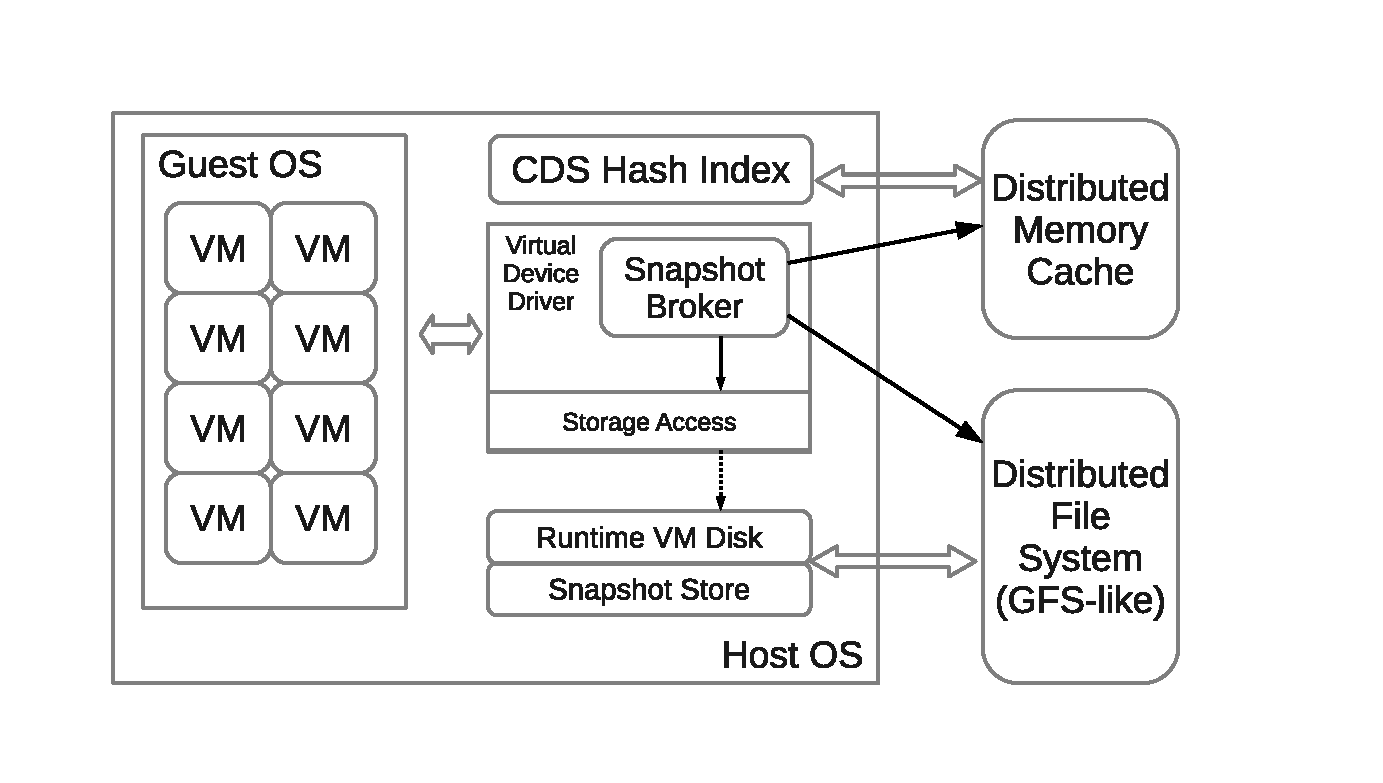
\epsfig{file=images/arch.eps, height=2in, width=2.66in}
  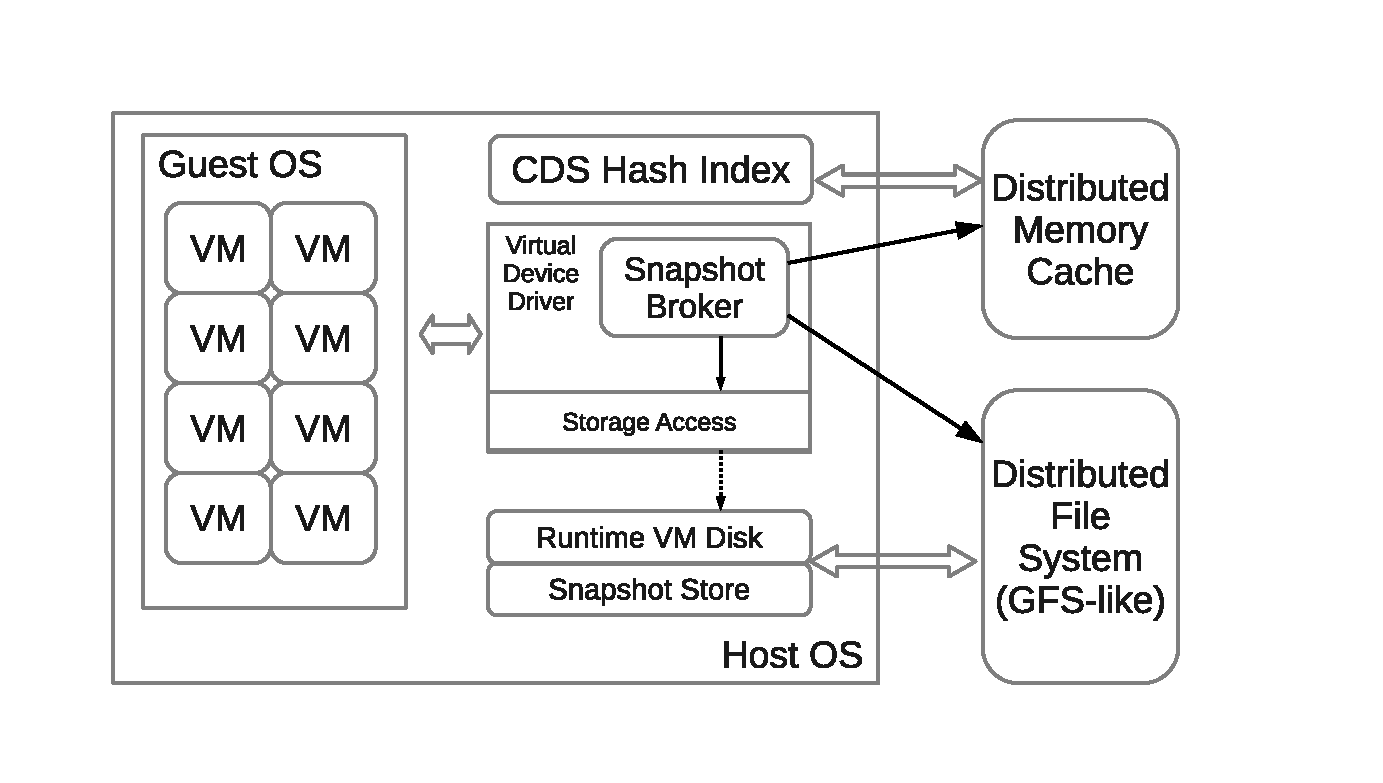
\epsfig{file=images/arch.eps, width=3.9in}
  \caption{Snapshot backup architecture of each node.}
  \label{fig:arch}
\end{figure}
The snapshot store 
supports data access operations such as \emph{get}, \emph{put} and \emph{delete}.
Other operations include data block traverse and resource usage report.
The snapshot data does not need to be
co-located with VM instances, and in fact they can even live in a different cluster to improve the 
data reliability: when one cluster is not available, we are still able to restore its VMs from another cluster which
holds its snapshot data. 
%to reduce the impact to our users.
%Get interface accepts a piece of data, write it to the underline data file, and return
%a reference to the caller. This reference then can be used in the put interface to
%retrive or delete the data, thus the caller of put interface must preserve the
%data reference for future use. 
%In addition to above standand data access operations, the snapshot service also supports
%\emph{scan} and \emph{quota} methods. Scan allows us to traverse all the data blocks of each VM
%in the snapshot store, and quota is used to acknowledge user how much space he
%has actually used.

Under the hood of snapshot store, it organizes and operates snapshot data 
in the distributed file system. We let each virtual disk has its own snapshot store, 
and no data is shared between
any two snapshot stores, thus achieve great fault isolation. For those selected popular data
that shared by many VM snapshot stores, we could easily increase its availability by having more replications.
%Since all the underline data structures is append only,
%upon a delete request, the corresponding data will only be marked rather than being deleted.
%A compaction will take place when deleted data has accumulated to a certain threshold, thus 
%reclaiming the disk space .


\subsection{Block Storage Device}
\subsection{CDS}
Although locality based data reduction can remove most of the inner-VM duplications,
it's not able to solve the data duplication cross VMs. Different VMs still share large amount
of common data such that their snapshot backups would have a lot of data in common.
Our observations on Aliyun's real VM user data reveals several major sources of cross-VM data duplication:
  \begin{enumerate}
  \item \emph{System-related data}: These data are generated by public third-parties, they are copied/downloaded/installed into VM disks either automatically or manually. Once installed, operations on such data are mostly read only until software updates arrive. For example, data of operating systems, some widely-used software such as Apache and MySQL, and their documations all fall into this category.
  \item \emph{User-generated data}: These data are generated by individual user's behavior, either directly or indirectly. They are much less duplicated than the system-related data, but the zipf-like distribution indicates that a small amount of data in this category could represent most of data duplications.
  \item \emph{Zero-filled data}: Like previous studies [refs here], we've observed that zero-filled data exist pervasively at system wide. They are almost like the spaces and commas in text articles. Under content-based chunking, they were distilled as zero-filled blocks with the maximum allowed length. 
%Zero-filled blocks are mostly generated by user behavior to preserve the space for future data, thus we treat them as a special case of user-generated data.
  \end{enumerate}

Without eliminating the data duplication between VM snapshot backups, storage space is severely wasted when the number of VMs increases.
To address this problem, we developed a technique called \emph{Common Data Set (CDS)} to eliminate data duplication for all three situations above. 
CDS is a public data library that shared by all VM snapshot backups in the cluster, 
which consists of the most popular data blocks in VM snapshot backups. It is generated, 
managed and accessed in an uniform manner by all VMs such that [write some fancy system characteristic stuff here].

\subsection{CDS Size V.S. Coverage}
As a shared data library, we expect CDS to collect almost all the system related data, the most popular user-generated data and the zero-filled data block.
With CDS as a public data reference, each VM's snapshot backup has no need to store its own copies for data that can be found in CDS, instead they can just
store a reference.

The more data we put into CDS, the closer we come to complete deduplication. But in reality we are facing a list of restrictions such like [blabla].
We borrowed the idea of web caching[refs here] to analysis the size of CDS vesus its effectiveness on data reduction.

We let $M$ be the number of nodes in a cluster, $N$ be the number of VMs hosted per node,
and let $D$ denotes the average size of one VM's snapshot backups (after level 1 and 2 reduction, which is near 40 GB in our production environment).
And let $C_0$, $C_s$ and $C_u$ denote the size of zero-filled block, system-related data and user-generated data in CDS,
then the total size of CDS is represented by $C=C_0+C_s+C_u$.
We let $S_0$, $S_s$ and $S_u$ denote the corresponding data coverage ratio (with respect to $D$) by $C_0$, $C_s$ and $C_u$,
so the total space saving ratio is $S=S_0+S_s+S_u$.

Zero-filled block at maximum length is the first item we need to put into CDS. This is the one and only special data block, 
and because CDS only stores unique data blocks, $C_0$ is almost equal to 0. In practice we found zero-filled blocks account
for near 20\% of total data, so $S_0$ is 20\%.

The rarely modified system-related data are the second to be added to CDS. We have thousands of VMs in each cluster, 
but all these VMs fall into only a few OS types, using a limited selection of software, therefore data duplication in this category
is highly noticable in a global block counting. In particular, most of such data already exist in the VM base images. 
We analyzed VMs running various services from 7 mainstream OS types in our cluster, and found close to 50GB of such data in total. 
Because system-related data don't change frequently, it's safe to expect that for 20 OS variations 
and software updates in 2 years, $C_s$ will not grow to exceed 200 GB.
For each VM, from 2 to 20 GB of data can be reduced in this way, depends on the OS and service type, so on average we estimate
$S_s$ would be no less than 20\%.

The rest of data are user-generated, the total size of such data can be written as $D_u=D-S_0-S_s$, which is 60\% of $D$. 
It follows a zipf-like distribution with $\alpha$ between 0.65 to 0.7. 
Let $T_u$ be the total size of unique data blocks in $D_u$,
in practice we notice that complete deduplication for such data always result in a 2:1 reduction ratio,
, so $T_u=D_u/2$.
Since we collect the most popular user-generated data into CDS, the coverage of CDS on user-generated data
is $(C_u/T_u)^{1-\alpha}$.

The following table lists CDS coverage on user-generated data under different $\alpha$ and $C_u/T_u$.

[a table of coverage with alpha from 0.65-0.70, ratio from 0.002 0.005 0.01 0.02 0.05]

It's obviously that at least 30\% of user-generated data can be reduced in this way, using about 0.02 of $T_u$, or 0.01 of $D_u$.
The size of user-generated data in CDS would be 0.006$D$, with coverage $S_u=0.18D$.

Thus the estimation of CDS coverage is $S=S_0+S_s+S_u=0.58$, with the size of CDS to be no more than $(200 + 0.006*D*N)$ GB.
In a VM cluster of 100 machines, with 25 VMs on each physical machine, the size of CDS is 800 GB in total, or 8 GB per machine.
The total size of CDS index would be 8 GB, which will cost 80 MB memory on each machine. 

\subsection{Append Store}
